\documentclass{book}
\usepackage{graphicx}
\begin{document}
\setcounter{chapter}{6}
\chapter{Managing the software project team}
\setcounter{section}{4}
\setcounter{subsection}{3}
\subsection{Recognition and Praise}

Another high motivator is giving recognition and praise to
members of your staff when their work is performed in an
exemplary manner. It essentially costs you nothing and takes
very little time to do, but it has a profound impact on the
work ethic of your staff. Most people love to have their ego
enhanced and the more often the better.
\textbf{Lessons Learned} I have worked for a few
(fortunately, very few) Managers who take
the approach of always looking for something
to complain about; Managers for whom you
cannot please no matter what you do. There is
nothing wrong with pushing your team to
excellence; however, when taken to an extreme
it is demoralizing to the team and is clearly the
wrong approach. This motivational factor is best
summed up by the poet Ella Wheeler Wilcox
who wrote: “A pat on the back is only a few vertebrae
removed from a kick in the pants, but is miles
ahead in results.”

\subsection{Job Enjoyment}

As long as I am quoting Ella Wheeler Wilcox, let me do one
more of her famous quotes: “Laugh and the world laughs
with you; weep and you weep alone.” Successful Software
Managers have the ability to loosen up, to enjoy working
with their staff, and can find ways to encourage their staff to
both work hard and play hard. In this context, “playing” can
mean having out-of-the-office games such as basketball or
soccer lunch breaks, pizza breaks (even better if the Manager
buys), company parties, brown bag lunches (also great for
learning sessions), holiday parties hosted by the Software
Manager and casual gatherings at the local waterhole after
work.

It is unreasonable to expect your staff to work hard
all the time. Outlets are forms of “play” that can pay large
dividends. The positive outcomes of these activities include
bonding friendships, promoting informal communications,
enhancing better health, making your project a fun place to
work and making you a terrific Manager.

\textbf{Lessons Learned} There are also some small,
inexpensive fun things you can do. For example,
I had a plastic figure of a funny looking guy
that you could punch on the head and he made
a burping noise. This 3.99dollar toy was revered by
my staff since each week it was awarded to the
best performer of the week, and it was proudly
displayed on the winner’s desk during the week.
It was once awarded to a senior member on my
staff just before he moved to another division of
the company and he insisted on taking the toy
with him (I gave it to him—and the two of them
rode off into the sunset).

Another good approach to enhancing job enjoyment
and increasing motivation is to provide food and snacks for
your team. Having a well-stocked refrigerator can provide
a priceless pay off in on-time product delivery because the
Developers can work productively together right through
dinner time and often well into the evening. When people
leave for dinner, they seldom return that evening. Some
larger firms even provide in-house catering to its technical
staff all day long.

\subsection{Personal Rewards}

It is generally agreed that Programmers are not highly
motivated by their paychecks, however, personal rewards
are important. In the high tech software world, this would
include salary increases, bonus, stock options, job promotions
and increased perks that collectively provide incentives
for higher performance. It is important to make sure that the
salaries received by your staff are fair and adequate. No one
will complain if the best Programmer on your staff is paid
the most. Salary and rewards to your staff should be fair, reasonable
and understandable. If your staff members feel fairly
compensated they will be focused on doing a good job and
salary becomes a non-issue.
Stock options for companies that have not yet gone public
can be a significant motivator, especially during recruiting.
The value of personal rewards is highly contingent on what is
important to each individual, so you have to determine what
motivates each person. In some cases, the right perk to the
right person may be the greatest impact to increasing their
motivation.

\subsection{Interpersonal Relationships}

A good interpersonal relationship usually means that staff
members will be much happier if they like the people they are
working with and for. If they really like the people they daily
interface with at work they will be motivated more than they
will be de-motivated if they don’t like them. Of course, if a
staff member simply can’t tolerate another staff member, you
have a problem that needs immediate attention. Software
Managers can and should take positive actions that can prevent,
or at least minimize, such problems.

Definitely avoid toxic people who are cynical and abrasive
as their negativity can be very disruptive. A serious mistake
a Manager can make is to tolerate any unacceptable
behavior that threatens team productivity. If you inherit such a person, you will likely need to work with HR to legally
eliminate that problem.

\textbf{Lessons Learned} During the hiring process,
here is one trick you can use to help identify
potential problems; propose the following scenario
to the candidate you are interviewing:
“Assume you are working on a project with
another Co-Developer, you are both fully qualified
to perform the required tasks, and you are
both at the same level of seniority.

There comes a point in the design process
where it is clear an innovative approach is needed
to solve a rather complex problem. You conceive
a creative solution that, in your judgment, will
fully solve the problem. However, your partner
has proposed a completely different approach
that you firmly believe is inferior to your solution.
How would you (the candidate) handle this
predicament?”

There is no one best answer to this question
because there are a few very good answers.
However, there is one wrong answer. If the candidate
firmly and resolutely insists on defending
his/her approach—no matter what—then you
can conclude this candidate is not very likely to
be a team player and stubborn enough to cause
dissension and disruption to the Development
Team. Almost any answer is okay except “my
way or the highway.”

You may find yourself working for a domineering
Senior Manager who believes that there are three ways to
perform a task: the right way, the wrong way, and his/her
way. If you subscribe to either of the first two approaches,
you are forevermore considered a “jerk” by that Manager.
Such a Manager believes that the only good ideas are his/
her ideas.

\textbf{Lessons Learned} One way to surreptitiously
get your domineering Manager to accept your
idea, or your approach to a solution, is to go
about it this way. In presentations to your
Senior Manager, and even during casual discussions
during lunch, lay out the problem, a
little at a time, in such a way that he/she will, on
their own, come up with the solution you have
in mind. When that happens, your response
should be “that is a great idea!” This works if
your Manager is analytical enough to follow a
structured thought process leading to the logical
conclusion. If your Manager does not think that
way… good luck.

\subsection{promotions}

The management of promotions can be tricky. It helps to
have good job descriptions but evaluating an employee’s performance
can be subjective and debatable when trying to
determine if an employee has demonstrated a level of performance
equal to or greater than what was expected for his/
her job. One common approach is not to promote someone
until they have already successfully performed at the level to
which they are being promoted.

This approach helps to avoid realization of The Peter
Principle—a management concept where the selection
of a candidate for a higher position is erroneously based
on their performance in their current role rather than on
their abilities relevant to the higher role. It is named after
Laurence J. Peter who co-authored the humorous 1969
book The Peter Principle: Why Things Always Go Wrong
(Peter and Hull, 2011). The author suggests that people
will tend to be promoted until they reach their level of
incompetence. The generalized Peter Principle is: Anything
that works will be used in progressively more challenging
applications until it fails. In other words, everyone and
everything has limitations.

The higher role that the employee is promoted to may
not be more difficult than the current role, but it may require
different skills the employee does not have. For example,
an excellent Programmer may prove to be a poor Manager
because of his/her limited interpersonal skills needed by a
Manager to lead a large team effectively. The following
guidelines can help to mitigate the risk associated with The
Peter Principle:

- Promote based on proof to succeed in the higher role
rather than the excellent performance demonstrated in
the lower-level current role. Progressively add tasks to
their current role that they will encounter in the higher
role and evaluate how well they performed them.

- If you must fill a role but you are not sure if the
employee you have selected to fill that role is capable
of handling it, you can put them in that role in an
“acting” status until they prove they can perform the
new tasks.

-Implement training programs in advance for those
being considered for promotion.

- Provide a parallel career path for your technical staff
without requiring their promotion to management,
similar to a warrant officer in the military.

-Implement an Up or Out approach, similar to policies
followed by the U.S. and British armed forces,
whereby persons not promoted above certain ranks,
within a fixed number of years, are deemed to lack
the necessary competence and are then discharged or
they resign.

\textbf{Lessons Learned} The last bullet reminds me
of Scott Adams’ humorous book, The Dilbert
Principle (Adams, 1996) where he proposes the
least smart people are promoted simply because
they’re the ones you don’t want doing actual work!
I once worked as a Software Lead on a large
software-intensive program where the Program
Manager was an old time hardware engineer who
called the software group a “cult.” After he did
sufficient harm to the program, they got rid of
him by promoting him to another smaller program
where he could do less harm. If you work
for such a Manager, hang in there until they
unravel enough rope to “hang themselves.”

It is interesting that some people seem to follow The Peter
Principle in reverse where their past performance and successes
are mediocre (or downright failures) until they achieve
a level of great importance and influence where they are
somehow inspired to achieve outstanding performance and
results. Abraham Lincoln may be an example of this as he
failed in most of his endeavors until he became an outstanding
President. We could call this the “Retep Principle” (Peter
in reverse).

\textbf{Lessons Learned}There is an old adage that
“failure is the mother of success.” There are
those who would consider the result a failure,
for what most people would judge as a reasonable
success if their task did not go exactly as
expected or planned. Such people are striving for
unreachable perfection. Sometimes, even if you
did everything perfectly, you may still encounter
failure for reasons beyond your control. If that
happens to you, always remember that losers stay
down, but winners get up, dust off and move on.

\subsection{ Working Conditions}

Most Software Managers have little control over the physical
working space for their staff since most companies have
standard space allocations and furniture selection choices.
Regardless, it is imperative that you provide the best possible
working environment for your staff so that they eagerly look
forward to going to work. You can allow your staff to personalize
their work area, you can provide ample conference
areas and whiteboards, and you can procure the best tools
and computer equipment to increase the productivity and
enjoyment of performing the work. As discussed in Section
9.6, offices with doors, even shared offices, for your technical
staff are far superior to cubicles but, realistically, you probably
have no choice if cubicles are the company standard.

\subsection{Technical Respect for Manager}

Having technical respect for the Manager is rated a low
impact as a motivator probably because it is expected that
employees would normally have such respect for their
Manager. However, if the employee does not have technical
respect for the Manager, then the impact as a cause for dissatisfaction
is very high. Software Managers must earn technical
respect from their staff and their peers.

If you are directly managing Programmers, you will have
a very difficult time managing them if you do not have a
very good understanding of the art of computer programming
as well as the related tools and processes. It also helps
to have a track record as a known and proven outstanding
Programmer or Software Engineer. In addition, you will
gain technical respect if you have made notable technical
contributions, or have advanced degrees, patents, certifications,
authored a book (who would want to do that?), active
membership in professional societies, and up-to-date with
the latest technical trends and technology.

In addition to earning technical respect, you also need to
earn personal respect and the best way to do that is to show
respect to your staff. If you treat them that way, they will treat
you that way in return. Showing respect can be demonstrated
in many ways including being a good listener, knowing the
names of each staff member and greeting them personally,
showing genuine interest by learning some things about their
non-work life, asking their opinions when appropriate, never
reprimanding publicly, and being courteous to them. This
may not be easy, especially for members of your staff that are
problematic but go out of your way to be respectful because
it will have a big payoff.

There are management gurus who claim that a Manager
should manage and not perform any technical work. My
view is that the percentage of time you should spend on management
tasks versus technical tasks depends on the size of
your program. If your project is small and you have a small
team, it is perfectly reasonable, and probably necessary, for
you to participate in the technical work, and your actual
responsibilities will be more of a “Programmer Lead” rather
than an SPM.

However, if you are managing a large complex softwareintensive
system, you may have little to no time to do any
real technical work. If you are an SPM, and performing a
substantial amount of technical work on your project, it is
almost a certainty that you are shortchanging your management
duties at the detriment of the entire project. My
notional guideline for the split of your time between management
and technical tasks is shown in Table 7.4.

As shown by the guidelines in Table 7.4, on a small project
you could spend an average of 80precent of your time performing
technical work; on a large project, you should not spend
more than 10precent of your time on technical tasks. If you find

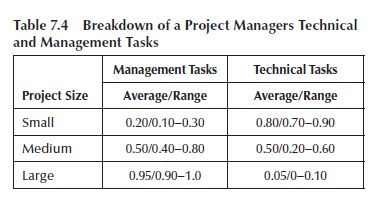
\includegraphics{1.jpg}

that your time distribution is outside these guidelines, you
should re-evaluate what it is you are doing versus what you
should be doing.

\subsection{Ethical and Realistic Policies}

As a Software Project Manager, you may not have much
influence on the ethical policies of your organization.
However, you must always act in an ethical and professional
manner. Being an ethical Manager means being honest and
sincere with your staff. Sometimes, unrealistic policies or
edicts come down from above and, if possible, you need to
intercept them before they reach your staff to avoid disruption
and distraction. Insulating your staff from these organizational
whiplashes may be necessary so that your Developers
can remain focused and productive.

When realistic changes do occur, they must eventually
be disseminated to your staff, but you can control the time
when the announcements are made to your team to avoid
interference with the completion of their project milestones.

\textbf{Lessons Learned}

It is usually easy to identify
unethical behavior; however, once in a while, the
distinction becomes hazy. If you are at a friend’s
party and he/she tells you something in a private
discussion about their company that is proprietary,
it is clearly unethical to relate this information
to your company because it is a violation of
their trust and friendship with you.

What is not so clear (to me) is an episode
that happened when I was working on a large
government proposal. I was eating lunch alone
in a quiet café and my table was against a half
wall down the middle of the café, topped with
plants that went halfway to the ceiling. Two men
sat down at a table on the opposite side of the
wall who were talking loud enough for anyone to
hear. They were working for a different company
on the same proposal, and they discussed topics
that should never be discussed in a public place.
When I returned to work, I told the Proposal Manager what I had heard. Later, I was told this was unethical! I am not sure I learned anything
from this episode because, to this day, I do not
believe I did anything unethical.

\section{Communications}

Communications is one of the most fundamental
skills of life and is a prerequisite to problem-solving.
Effective communication is a cornerstone to successful
project management.

Abraham Lincoln once said “Not saying anything and being
thought of as a fool is better than opening your mouth and
removing all doubt.” Sure, there are times when remaining
silent is the wise choice, but an effective Project Manager
must also be an effective communicator. Although good
communications is not rated as a high motivator, it is an
important de-motivator if your team members feel they are
“out of the loop” and not connected to what is going on. If
that is the case, it is a problem you must solve. The following
is a personal example of how a lack of project related communications
can be a serious de-motivator.

\textbf{Lessons Learned} I was the Lockheed Software
Group Lead on the NASA Space Station Freedom
program on one of the subsystems (called work
packages) where Lockheed was a subcontractor
to another major aerospace company; they were
the prime contractor for our work package. They
had frequent meetings and telephone conferences,
and good email communications, so all
of the subcontractors participated, and everyone
knew what was going on—it was a full team effort.
Everyone was enthusiastic and productive.
Meanwhile, in another part of our building,
there was an additional Software Team working
on a different Space Station work package. They
were also a subcontractor to a different aerospace
company, the prime contractor for their subsystem,
who kept them almost totally in the dark.
Their prime contractor had infrequent meetings
and a very serious lack of communication. It is an
understatement to say that this Software Team
was frustrated and they were not even close to
the productivity of my team. They came to me to
find out what was going on regarding the overall
program.

Both of these prime contractors are large
aerospace firms with a long legacy. This experience
was an education in the cultural differences
in management style by two mature companies in the same industry. The lesson here is you have
to expect to encounter, and learn to cope with,
extremes in management style.
The importance of communications, and the approaches
to enhancing communications in your project, is further
illustrated in the following four discussions on the root
cause of problems, the importance of honest discussions,
the exponential growth in lines of communication as the
size of your team expands, and some methods to cultivate
communication.

\subsection{Root Cause of Problems}

The lack of good communications is often the root cause of
management problems in many organizations. Developers
need to accept the results of others, and they must communicate
their ideas and results verbally and preferably with
written documentation. Constructive criticism of software
development work products is needed and should be encouraged—
as long as it is offered in a calm, professional, respectful
and non-accusatory fashion.

As the Project Manager, you must communicate regularly
and frequently with Software Developers and other stakeholders.
Frequent communication is a very important factor
in increasing the likelihood of project success and the mitigation
of problems. The Development Team should always seek
customer and/or end-user involvement and encourage enduser
input in the development process. Not having customer
and/or end-user involvement can lead to misinterpretation of
requirements, insensitivity to changing customer needs, and
unrealistic customer expectations.

Digging for the root cause of problems is another important
task for Project Managers. The symptoms of a problem
are usually easy to see, but the root cause is usually hidden.
The problem you see and hear is at the surface; you need to
dig deeper to find the real root cause. Keep communicating
whenever you encounter dysfunctional behavior because if
you don’t resolve the problem, it can grow in intensity to a
point where it may be too late, or too big, to fix.

\subsection{Honest Discussions}

Intellectually honest discussions provide an opportunity to
analyze strengths, weaknesses and pitfalls, and to act on
that information to minimize potential problems. Even bad
news can be helpful if communicated relatively early so that
timely Corrective Action can be taken. Casual conversations
with users, team members, and other stakeholders may surface
potential problems sooner than made known at formal
meetings, and they help keep the project timely, relevant and
within the bounds of what can realistically be completed in
a given time period.

\subsection{Lines of Communication}
Progress of your project is highly dependent on the effectiveness
and the ability of the team members to communicate
with each other as well as with end-users and other stakeholders.
Software failures can result from a breakdown in understanding,
so the ability of people to communicate with one
another can easily affect the quality of the product. The reality
of this serious problem becomes clear when you realize
that the lines of communication increase exponentially as your
staff grows larger. This exponential increase is demonstrated
by the formula:
L = S(S–1)/2 where “L” is Lines of communication and “S”
is the “Size” of your staff.
Table 7.5 shows the results of this compounding communications
problem that you must consider and resolve if
you have a large staff.

\subsection{Cultivate Communication}

\textit{If everyone is thinking alike, then somebody isn’t
thinking.}

\textbf{—George S. Patton (1885–1945)}

There are many ways to foster better communications up,
down and across an organization. In larger companies,
there should be periodic (often quarterly) all hands meetings,
monthly departmental meetings and written communication
in the form of bulletins, newsletters, memorandum
and email. But for your team, you should (maybe must)
have weekly staff meetings, brown bag lunch meetings and
off-site meetings.
Also, you should monitor gossip since that can be a major
distraction. I read about a Manager that would open his staff
meetings with an invitation to share gossip. When part of
your team is geographically disbursed, effective communications
becomes even more critical, and it is your responsibility
to ensure that needed information is flowing to your team
regardless of location.

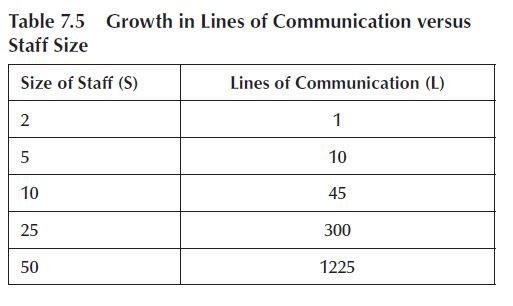
\includegraphics{2.jpg}
\end{document}